\documentclass[12pt]{report} % Increased the font size to 12pt
\usepackage{epigraph}
\usepackage{geometry}

% Optional: customize the style of epigraphs
\setlength{\epigraphwidth}{0.5\textwidth} % Adjust the width of the epigraph
\renewcommand{\epigraphflush}{flushright} % Align the epigraph to the right
\renewcommand{\epigraphrule}{0pt} % No horizontal rule
\usepackage[most]{tcolorbox}
\usepackage{amsmath, amssymb, amsthm}
\usepackage{bbm}
\usepackage{graphicx}
\usepackage{caption}
\usepackage[utf8]{inputenc}
\usepackage{hyperref} % Added for hyperlinks
\usepackage{listings} % Added for code listings
\usepackage{color}    % Added for color definitions
\usepackage[super]{nth}
\usepackage{fancyhdr}
\usepackage{tikz}
\usepackage{cite}
\usepackage{algpseudocode}
\usetikzlibrary{shapes.geometric, arrows, positioning}

\tikzstyle{startstop} = [rectangle, rounded corners, minimum width=3cm, minimum height=1cm, text centered, draw=black, fill=red!30]
\tikzstyle{io} = [trapezium, trapezium left angle=70, trapezium right angle=110, minimum width=3cm, minimum height=1cm, text centered, draw=black, fill=blue!30]
\tikzstyle{process} = [rectangle, minimum width=3cm, minimum height=1cm, text centered, draw=black, fill=orange!30]
\tikzstyle{decision} = [diamond, minimum width=3cm, minimum height=1cm, text centered, draw=black, fill=green!30]
\tikzstyle{arrow} = [thick,->,>=stealth]

% Define the graphics path
%\graphicspath{{./Plots/}}

% Define the header and footer for general pages
\pagestyle{fancy}
\fancyhf{} % Clear all header and footer fields
\fancyhead{} % Initially, the header is empty
\fancyfoot[C]{\thepage} % Page number at the center of the footer
\renewcommand{\headrulewidth}{0pt} % No header line on the first page of chapters
\renewcommand{\footrulewidth}{0pt} % No footer line

% Define the plain page style for chapter starting pages
\fancypagestyle{plain}{%
  \fancyhf{} % Clear all header and footer fields
  \fancyfoot[C]{\thepage} % Page number at the center of the footer
  \renewcommand{\headrulewidth}{0pt} % No header line
}

% Apply the 'fancy' style to subsequent pages in a chapter
\renewcommand{\chaptermark}[1]{%
  \markboth{\MakeUppercase{#1}}{}%
}

% Redefine the 'plain' style for the first page of chapters
\fancypagestyle{plain}{%
  \fancyhf{}%
  \fancyfoot[C]{\thepage}%
  \renewcommand{\headrulewidth}{0pt}%
}

% Header settings for normal pages (not the first page of a chapter)
\fancyhead[L]{\slshape \nouppercase{\leftmark}} % Chapter title in the header
\renewcommand{\headrulewidth}{0.4pt} % Header line width on normal pages

\setlength{\headheight}{14.49998pt}
\addtolength{\topmargin}{-2.49998pt}
% Define colors for code listings
\definecolor{codegreen}{rgb}{0,0.6,0}
\definecolor{codegray}{rgb}{0.5,0.5,0.5}
\definecolor{codepurple}{rgb}{0.58,0,0.82}
\definecolor{backcolour}{rgb}{0.95,0.95,0.92}

% Setup for code listings
\lstdefinestyle{mystyle}{
    backgroundcolor=\color{backcolour},
    commentstyle=\color{codegreen},
    keywordstyle=\color{magenta},
    numberstyle=\tiny\color{codegray},
    stringstyle=\color{codepurple},
    basicstyle=\ttfamily\footnotesize,
    breakatwhitespace=false,
    breaklines=true,
    captionpos=b,
    keepspaces=true,
    numbers=left,
    numbersep=5pt,
    showspaces=false,
    showstringspaces=false,
    showtabs=false,
    tabsize=2
}

\lstset{style=mystyle}

% Definition of the tcolorbox for definitions
\newtcolorbox{definitionbox}[1]{
  colback=red!5!white,
  colframe=red!75!black,
  colbacktitle=red!85!black,
  title=#1,
  fonttitle=\bfseries,
  enhanced,
}

% Definition of the tcolorbox for remarks
\newtcolorbox{remarkbox}{
  colback=blue!5!white,     % Light blue background
  colframe=blue!75!black,   % Darker blue frame
  colbacktitle=blue!85!black, % Even darker blue for the title background
  title=Remark:,            % Title text for remark box
  fonttitle=\bfseries,      % Bold title font
  enhanced,
}

% Definition of the tcolorbox for examples
\newtcolorbox{examplebox}{
  colback=green!5!white,
  colframe=green!75!black,
  colbacktitle=green!85!black,
  title=Example:,
  fonttitle=\bfseries,
  enhanced,
}

% Definitions and examples will be put in these environments
\newenvironment{definition}
    {\begin{definitionbox}}
    {\end{definitionbox}}

\newenvironment{example}
    {\begin{examplebox}}
    {\end{examplebox}}

\geometry{top=1.5in} % Adjust the value as needed
% ----------------------------------------------------------------------------------------


\title{S2 Statistics for Data Science}
\author{CRSiD: tmb76}
\date{University of Cambridge}

\begin{document}

\maketitle

\tableofcontents

\chapter*{The Lighthouse Problem}

\chapter{The Setup}

\indent A lighthouse that is at a distance $\beta$ from the coast is at position $\alpha$ along it. The lighthouse emits flashes at random angles $\theta$, following a uniform distribution. The flashes can be considered narrow and, provided $\pi/2 < \theta < \pi/2$, intersect the coastline at a single point. Detectors on the coastline record only the flashes' locations $x_{k}$ and their intensity $I_{k}$ (where $k = 1, 2,\dots, N$ ) for N flashes received. The setup is illustrated in Figure \ref{fig:lighthouse}.

\begin{figure}[h]
\centering
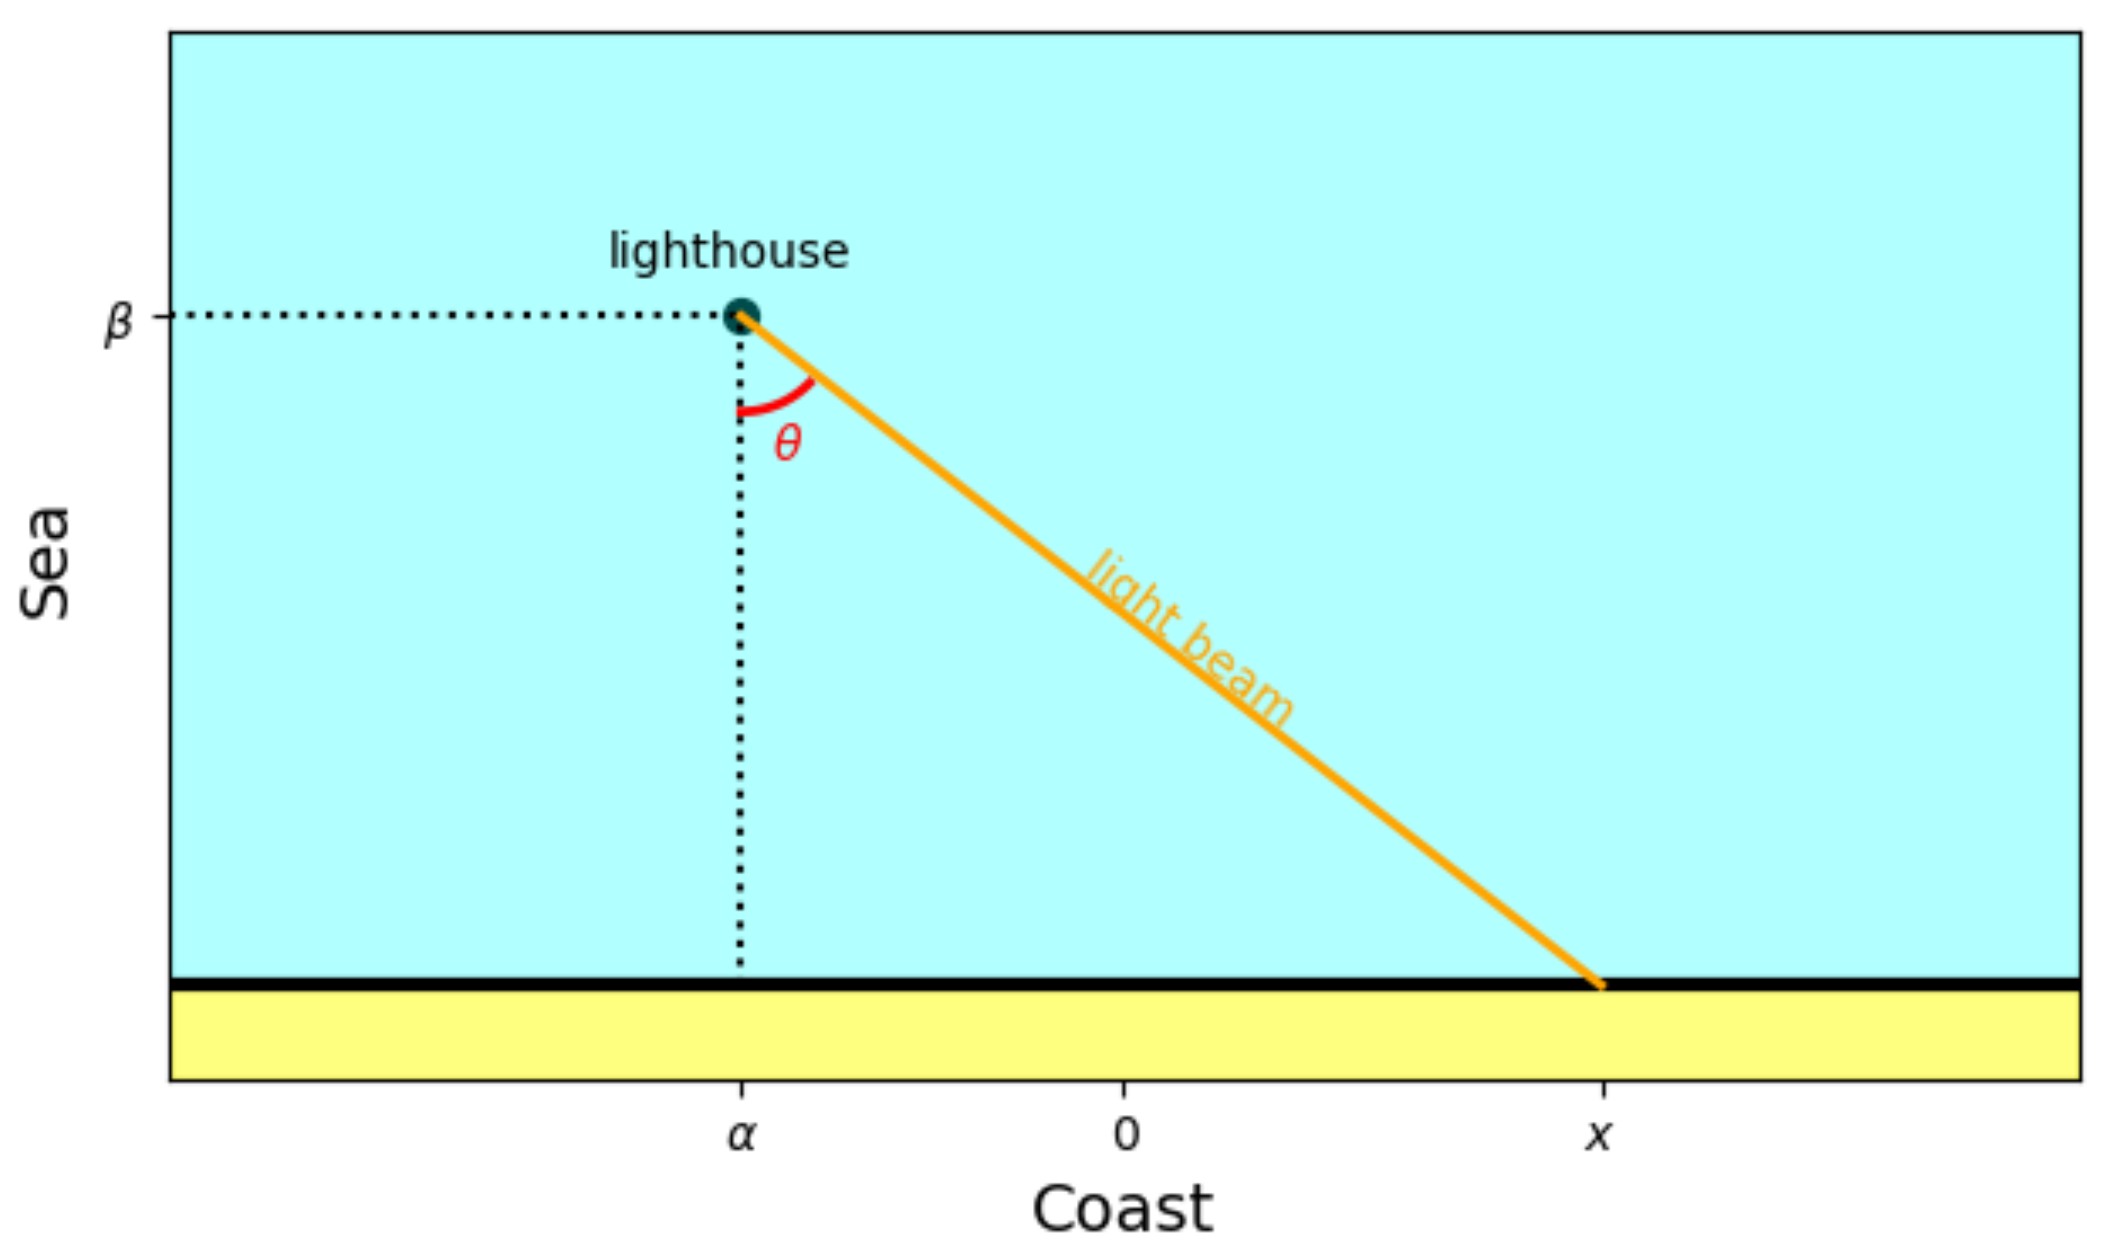
\includegraphics[width=0.8\textwidth]{../Plots/lighthouse diagram.png}
\caption{The lighthouse problem setup}
\label{fig:lighthouse}
\end{figure}


The goal of this project is to find the location of the lighthouse using the observed detector data $\{x_{k}\}$, and $\{I_{k}\}$ and their known likelihood.

\chapter{(i) The Geometry of the Problem}

As stated above, only the distribution of the flashes' angle, $\theta$, is known. However, the observed data obtained is the location of the flashes on the coastline, $x_{k}$. Thus, it is worth considering what the relationship is between the angle of the flash and the location of the flash on the coastline, expressed in terms of the unknown lightouse location parameters $\alpha$ and $\beta$. Using trigonometry, the following relationship can be derived:

\begin{equation}
    x = \alpha + \beta \tan(\theta) \iff \theta = \tan^{-1}\left(\frac{x - \alpha}{\beta}\right)
\end{equation}

\chapter{(ii) The Likelihood Function}

In addition to the relationship above, the probability distribution of the flashes' angles is known to be uniform. Thus, the probability of a single flash to have the angle $\theta$ is given by\cite[p.79]{FJames2006}:

\begin{equation}
    \theta \sim U(-\pi/2, \pi/2)
\end{equation}

\begin{equation}
    P(\theta) = \mathbbm{1}_{(-\pi/2, \pi/2)}(\theta) \times \frac{1}{\pi} = \begin{cases} \frac{1}{\pi}, & \text{if } -\frac{\pi}{2} < \theta < \frac{\pi}{2} \\ 0, & \text{otherwise} \end{cases}
\end{equation}

Now, using the trigonometric relationship between $\theta$ and $x$ derived in (1), a change of variable is conducted to find the probability distribution of the flashes' locations on the coastline, $x$. Here, this will be considered as the likelihood of a single flash to be observed at location $x$ given the lighthouse location parameters $\alpha$ and $\beta$. For this 1-D case, the change of variable can be written as\cite[p.20]{FJames2006}:

\begin{equation}
    \mathcal{L}_{x}(x|\alpha, \beta) = \mathcal{L}_{\theta}(\theta) \times \left| \frac{d\theta}{dx} \right|
\end{equation}

Where $\mathcal{L}_{\theta}(\theta)$ is the probability distribution of the flashe's angles, which is given in Eq (3) as a uniform distribution. Since the angle $\theta$ must be such that $-\pi/2 < \theta < \pi/2$ for the flash to be observed on the coastline, $\mathcal{L}_{\theta}(\theta)$ can be set to $1/\pi$. The derivative term is given by:

\begin{equation}
    \frac{d\theta}{dx} = \frac{d}{dx} (\tan^{-1}\left(\frac{x - \alpha}{\beta}\right) )
\end{equation}

Using the chain rule, the derivative can be found to be:

\begin{equation}
    \frac{d\theta}{dx} = \frac{1}{1 + \left(\frac{x - \alpha}{\beta}\right)^{2}} \times \frac{1}{\beta}
\end{equation}

With some algebraic manipulation, this can be re-arranged as:

\begin{equation}
    \frac{d\theta}{dx} = \frac{\beta}{\beta^{2} + (x - \alpha)^{2}}
\end{equation}

Thus the likelihood for a single flash to be observed at location $x$ given the lighthouse location parameters $\alpha$ and $\beta$ is:

\begin{equation}
    \mathcal{L}_{x}(x|\alpha, \beta) = \frac{1}{\pi} \times \frac{\beta}{\beta^{2} + (x - \alpha)^{2}}
\end{equation}

as required. Below is an example plot of the likelihood function for hypothetical values of $\alpha = 0$ and $\beta = 1$.

\begin{figure}[h]
\centering
\includegraphics[width=0.8\textwidth]{../Plots/lighthouse_cauchy_distribution.png}
\caption{Cauchy distribution plot, for hypothetical values of $\alpha = 0$ and $\beta = 1$}
\label{fig:cauchy_distribution}
\end{figure}

Fig. \ref{fig:cauchy_distribution} shows the Cauchy distribution, which is a heavy-tailed distribution \cite[p34]{sivia_data_analysis} \cite[p84]{FJames2006}. This means that the likelihood stays non-negligible for values of x very different from $\alpha$. This can be understood from the trigonometric relationship between $\theta$ and $x$ in Eq. (1). When the angle $\theta$ is close to $\pm \pi/2$, small changes in $\theta$ result in large changes in $x$. And since the angle $\theta$ is uniformly distributed, the likelihood of observing a flash at a location $x$ far from $\alpha$ stays non-negligible.

\chapter{(iii) Frequentist Claim}

A frequentist colleague claims the most likely location, $\hat{x}$, for any flash to be received is given by the parameter $\alpha$, the location of the lighthouse along the coastline. They also suggest using the sample mean to estimate the $\alpha$ parameter. First, the $\hat{x} = \alpha$ claim. $\hat{x}$ is, by definition, the location for which the likelihood in Eq. (8) is maximised. This is found by taking the derivative of the likelihood with respect to $x$ and setting it to zero. This gives:

\begin{equation}
    \left. \frac{d\mathcal{L}_{x}(x|\alpha, \beta)}{dx} \right|_{x = \hat{x}} = 0 \iff \left. \frac{d}{dx} \left(\frac{\beta}{\beta^{2} + (x - \alpha)^{2}}\right) \right|_{x = \hat{x}} = 0
\end{equation}

\begin{equation}
    -\frac{1}{\pi} \beta (2\hat{x} - 2\alpha)\frac{1}{\beta^{4} + 2\beta^{2}(\hat{x} - \alpha)^{2} + (\hat{x} - \alpha)^{4}} = 0
\end{equation}
\newline
The $-\frac{1}{\pi} \beta$ terms can be dropped, leaving only the numerator $(2\hat{x} - 2\alpha)$ term to be equal to 0 to satisfy the equation. This is done when $\hat{x} = \alpha$, as claimed. Thus, the frequentist's claim is accurate for the value of the most likely flash location. However, estimating the value of $\alpha$ with the sample mean is not robust. To show this, the Maximum Likelihood Estimate (MLE) method is used to compare the two estimators \cite[pp 135-137]{FJames2006}. The aim is to find the value of $\alpha$ that maximises the likelihood derived in Eq. (8), based on the observed sample $\{x_k\}$ ($k = 1, 2,\dots, N$). This means now having the likelihood being the product of individual likelihoods for all values of $\{x_k\}$, as the flashes are emitted at independent angles. Finding $\hat{\alpha}$ is done in a similar way as above, by taking the derivative of the likelihood with respect to $\alpha$ this time and setting it to zero. However, for simplicity in derivation and computation, the log-likelihood is used instead.

\begin{equation}
    \hat{\alpha}_{MLE} = \arg \max_{\alpha} \ln(\prod_{k=1}^{N}  \mathcal{L}_{x}(\{x_{k}\}|\alpha, \beta)) = \arg \max_{\alpha} \sum_{k=1}^{N} \ln(\frac{1}{\pi} \times \frac{\beta}{\beta^{2} + (x_{k} - \alpha)^{2}})
\end{equation}

\begin{equation}
    \hat{\alpha}_{MLE} = \arg \max_{\alpha} \sum_{k=1}^{N} \ln(\frac{\beta}{\pi}) + \ln(\frac{1}{(\beta^{2} + (x_{k} - \alpha)^{2})})
\end{equation}

\begin{equation}
    \left. \frac{d}{d\alpha} \left( \sum_{k=1}^{N} \ln(\frac{\beta}{\pi}) - \ln(\beta^{2} + (x_{k} - \alpha)^{2}) \right) \right|_{\alpha = \hat{\alpha}_{MLE}} = 0
\end{equation}

\begin{equation}
    \sum_{k=1}^{N} \frac{(2\hat{\alpha}_{MLE} - 2x_{k})}{\beta^{2} + (x_{k} - \hat{\alpha}_{MLE})^{2}} = 0
\end{equation}
\newline
To get an estimate of $\hat{\alpha}_{MLE}$, the above equation needs to be rearranged to isolate $\alpha$. However, this is difficult to do analytically. The sample mean estimator can be tested numerically\cite[p. 32]{sivia_data_analysis}. Using Pedro Pessoa's example code for the lighthouse problem \cite{pessoa_lighthouse}, flash location sample data is generated for hypothetical $\alpha = 2$ and $\beta = 2$. The sample mean and confidence intervals are then calculated and compared to the true mean. The results are shown in Fig. \ref{fig:sample_mean} and are similar to the example shown in Fig 2.9 of Section 2.4 in Silvia's book \cite{sivia_data_analysis}.

\begin{figure}[h]
\centering
\includegraphics[width=0.8\textwidth]{../Plots/cauchy_CLT.png}
\caption{Plot of smaple mean and confidence intervals for the lighthouse problem, for varying sample sizes, with true parameters set to $\alpha = 2$ and $\beta = 2$}
\label{fig:sample_mean}
\end{figure}

Fig. \ref{fig:sample_mean} shows that the sample mean estimator is not consistent as it does not converge with the sample size increasing\cite[p.128]{FJames2006}, sometimes even getting worse. This is due to the heavy-tailed nature of the Cauchy distribution  \cite[p34]{sivia_data_analysis} \cite[p84]{FJames2006}. And in the context of the lighthouse problem, the physical explanation for this was discussed shortly at the end of section (ii). The overarching issue is that the Cauchy distribution does not follow the Central Limit Theorem (CLT) \cite[p34]{sivia_data_analysis}. This is because the mean, or expected value of the cauchy distribution is undefined \cite[p84]{FJames2006}. This is shown in James' book \cite[p34]{FJames2006} where the characteristic function of the Cauchy distribution has no derivatives at t=0, which from the definition of the central moment, means it has no defined mean:

\begin{equation}
    \frac{d}{dt}\phi(t) = \frac{d}{dt}\int_{-\infty}^{\infty} e^{itx} \frac{1}{\pi} \frac{\beta}{\beta^{2} + (X - \alpha)^{2}} dX = \text{Undefined}
\end{equation}


\chapter{(iv) Priors for $\alpha$ and $\beta$}

Since a prior distribution's primary goal is to describe how much we know about the parameters before observing the data\cite[p.154]{FJames2006}. For the lighthouse problem, it is only known that the lighthouse is at some location $\alpha$ along the coastline and at some distance $\beta$ from the coastline. Thus, the priors for $\alpha$ and $\beta$ should be ignorant ones, such as the uniform distribution. And even though there are the 20 measured $\{x_{k}\}$ samples that could back the use of a normal distribution about the sample mean with large variance, section (iv)'s discussion discourages this. These can be written as\cite[p.79]{FJames2006}:

\begin{equation}
    \alpha \sim U(\alpha_{min}, \alpha_{max}) \text{ and } \beta \sim U(0, \beta_{max})
\end{equation}

\begin{equation}
    P(\alpha) = \mathbbm{1}_{(\alpha_{min}, \alpha_{max})}(\alpha) \times \frac{1}{\alpha_{max} - \alpha_{min}} \text{ and } P(\beta) = \mathbbm{1}_{(0, \beta_{max})}(\beta) \times \frac{1}{\beta_{max}}
\end{equation}

where $\mathbbm{1}$ is the indicator function. $\beta$ is non-negative, hence the lower bound of the uniform distribution for $\beta$ is 0.


\chapter{(v) Stochastic Sampling }

\section{Defining the Posterior}

With the likelihood and priors defined, and the general lighthouse problem understood, estimating the location parameters $\alpha$ and $\beta$ can be attempted. Here stochastic sampling approaches are used, directly drawing samples from the posterior distribution of the parameters. The posterior distribution is given by Bayes' theorem as:

\begin{equation}
    P(\alpha, \beta | x) = \frac{\mathcal{L}_{x}(x | \alpha, \beta) \times \pi(\alpha,\beta)}{Z}
\end{equation}

where $\pi(\alpha,\beta)$ is the joint prior distribution of $\alpha$ \& $\beta$, and $Z$ is the evidence \cite[p.6]{sivia_data_analysis}. The evidence is the normalising constant, which is the integral of the likelihood function over the entire parameter space\cite{knuth_bayesian_evidence}\cite{slideserve_bayesian_evidence}. Since it is a constant, evaluating it is not necessary for the purposes of sampling values of $\alpha$ and $\beta$ from the posterior, i.e. it is only important that $P(\alpha, \beta | x) \propto \mathcal{L}_{x}(x | \alpha, \beta) \times \pi(\alpha,\beta)$. Furthermore, the joint prior distribution $\pi(\alpha,\beta)$ is simply the product of the individual priors for $\alpha$ and $\beta$, as they are independent. Finally, the estimation of the location parameters $\alpha$ and $\beta$ is based on $N = 20$ observed flash locations. These observations are plotted in Fig. \ref{fig:observations}'s diagram.

\begin{figure}[h]
\centering
\includegraphics[width=0.8\textwidth]{../Plots/lighthouse_flashes_diagram.png}
\caption{The observed flash locations on the coastline, with a hypothetical lighthouse location at $\alpha = 0$ and $\beta = 0.1$}
\label{fig:observations}
\end{figure}

\newpage

With these data points, the likelihood in Eq. (18) is the product of the likelihood for each observation as in Eq. (11). This means the posterior distribution, $P$, can be rewritten as:

\begin{equation}
    P(\alpha, \beta | \{x_{k}\}) \propto \mathcal{L}_{x}(\{x_{k}\} | \alpha, \beta) \times \pi(\alpha) \times \pi(\beta)
\end{equation}

Giving the following expression:

\begin{equation}
    P(\alpha, \beta | \{x_{k}\}) \propto (\frac{\beta}{\pi})^{N} \times \prod_{k=1}^{N}\frac{1}{(\beta^{2} + (x_{k} - \alpha)^{2})} \times \frac{1}{\beta_{max}(\alpha_{max} - \alpha_{min})}
\end{equation}

Finally, for numerical precision reasons, to avoid product of small numbers in the code, the log posterior is used instead:

\begin{equation}
    \ln(P(\alpha, \beta | \{x_{k}\})) \propto N\ln(\beta) - N\ln(\pi) - \sum_{k=1}^{N}\ln(\beta^{2} + (x_{k} - \alpha)^{2}) - \ln(\beta_{max}) - \ln(\alpha_{max} - \alpha_{min})
\end{equation}

Since the natural logarithm is a one-to-one mapping and is invertible, this will not affect the final result of the sampling, i.e. estimates of $\alpha$ and $\beta$.

\section{Sampling Methods}

Here, multiple Markov Chains Monte-Carlo (MCMC) sampling algorithms were used. The first is the Metropolis-Hastings (MH) algorithm described below\cite{ravenzwaaij_markov_chain}. One of the good things of the MH algorithm is that it does not require us to know the normalised target distribution.

\begin{definitionbox}{Metropolis-Hastings Algorithm}
    \begin{algorithmic}[1]
        \State $l_{0} \sim (\alpha, \beta)$ \Comment{Initialisation}
        \State $i \gets 0$
        \While{$i \geq 0$} \Comment{Iterate $i = 0, 1, \dots, N$}
            \State $y \sim \mathcal{N}(\alpha, \beta | l_{i}, cov)$ \Comment{Proposal distribution, here, a multivariate normal}
            \State $a \gets (P(y|\{x_{k}\})\mathcal{N}(l_{i}|y, cov))/(P(l_{i}|\{x_{k}\})\mathcal{N}(y|l_{i}, cov))$ \Comment{MH acceptance probability}
            \State $u \sim U(0, 1)$ \Comment{Uniform random number}
            \If{$u < a$}
                \State $l_{i+1} \gets y$ \Comment{Accept the proposal}
            \Else
                \State $l_{i+1} \gets x_{i}$ \Comment{Reject the proposal}
            \EndIf
            \State $i \gets i + 1$
        \EndWhile
        \end{algorithmic}
    Where $cov$ is the covariance matrix of the multivariate normal distribution, $P(l_{i}|\{x-{k}\})$ is the posterior distribution, and $l, y = (\alpha, \beta)$ are proposed points in the parameter space.
\end{definitionbox}

\vspace*{1\baselineskip}
The key step of MH, line 7 of the algorithm, is the check of the acceptance probability, $a$. This is the ratio of the posterior distribution at the proposed point, $y$, to the posterior distribution at the current point, $l_{i}$, multiplied by the ratio of the proposal distribution at the current point, $l_{i}$, to the proposal distribution at the proposed point, $y$. The proposal distribution is a multivariate normal distribution, with mean $l_{i}$ and covariance matrix $cov$, which is to be chosen. Here, the covariance will be diagonal, so no covariance between $\alpha$ and $\beta$. The acceptance probability is then implemented by sampling a uniform number between 0 and 1, therefore the condition on line 7 being satisfied has a probability of occuring $a$. If the acceptance probability is greater than $u$, the proposed point is accepted, and the chain moves to the proposed point. Otherwise, the proposed point is rejected, and the chain stays at the current point. The chain then iterates, moving through the parameter space, until a sufficient number of samples are obtained. One downside to MH is that it can be slow to converge\cite{li_monte_carlo}, and line 10 of the algorithm makes it so MH can stay at the same point for multiple iterations, resulting in repeated samples.


Second, the slice sampling algorithm is used. This algorithm is also a MCMC algorithm and follows a relatively simple procedure. The main idea is to sample uniformly from the region under the curve of the posterior distribution. One of the main advantages of slice sampling is that it's acceptance rate is always 1, meaning that it is very efficient. Furthermore, where the MH algorithm requires some tuning thought, with the proposal distribution and its covariance matrix here, slice-sampling only requires the posterior\cite{neal_slice_sampling}. Again, the slice sampling algorithm is described below.\cite{karamanis_zeus}

\begin{definitionbox}{Slice Sampling Algorithm \cite{karamanis_zeus}}
\fontsize{8}{12}\selectfont
    \begin{algorithmic}[1]
        \State Initialize:
        \State \quad $l_0 \gets$ Initial state
        \State \quad $i \gets 0$
        \While{$i \geq 0$} \Comment{Iterate until desired number of samples}
            \State $y_{0} \sim U(0, P(l_{i}|\{x_{k}\}))$
            \State Stepping Out Procedure: To find $I = (L, R)$ that contains all or at least part of $S$, expand I by a step of size $\mu$ until both ends of $I$: $L$ and $R$ are outside of $S$
            \State $l_{i+1} \sim U(I \cap S)$ \Comment{Shrinking Procedure: Sample $l_{i+1}$ from I until one of them is inside S}
            \State $i \gets i + 1$
        \EndWhile
    \end{algorithmic}
    Where $S$ is the slice for which $\{l: y_{0} < (l_{i}|\{x_{k}\})\}$, and $P(l_{i}|\{x_{k}\})$ is the posterior distribution.
\end{definitionbox}

\vspace*{1\baselineskip}
The issue that arises with simple slice sampling here is that the stepping out procedure has no guarantee of finding the entire slice S, especially in case of multimodal distributions. This is where the software package used, \texttt{zeus}, comes in. \texttt{zeus} is a Python package that implements a more sophisticated version of slice sampling, called Ensemble Slice Sampler. As its name suggests, it uses an ensemble of walkers to sample from the posterior distribution, each with a different starting point. This minimises the chances of the total chain sampled missing an entire mode of the posterior distribution \cite{karamanis_zeus}. However, one issue is that setting a random seed for this package is tricky, and so the results may vary between runs, though they should stay consistent, and the comparison between the two sampling methods should still be valid.


\section{Results}

\subsection{Metropolis-Hastings}


The total acceptance fraction for the chain was 0.27555, which is reasonable for the MH algorithm\cite{metropolis_hastings}\cite{bedard_optimal_acceptance_rates}. In order to reflect the a priori knowledge we had of the position of the lighthouse, the initial position of the chain was set randomly, following a uniform distribution in between the set limits. It could be argued to start the $\alpha$ parameter at the sample mean value of the 20 observations. However, this is again discouraged by the cauchy distribution and the fact that the a priori knowledge was set to be ignorant. Regardless, the $\beta$ parameter certainly must be set randomly. This means the chain would have to converge first to the region of high probability, which requires us to ignore the first few samples of the chain \cite{ravenzwaaij_markov_chain}. To check how many samples it took for the chain to converge, a plot of the first 1500 samples was made.

\begin{figure}[h]
\centering
\includegraphics[width=0.8\textwidth]{../Plots/chain_plot_vMH.png}
\caption{First 1500 samples of the MH chain for the lighthouse problem}
\label{fig:MH_convergence}
\end{figure}

Fig. \ref{fig:MH_convergence} shows that the chain converges in just about 1500 steps. Thus, before estimating the parameters from the chain, this burn-in period of 1000 steps must be ignored and dropped. Furthermore, once this is done, due to the nature of MCMC chains, subsequent samples are correlated \cite{vandeschoot_bayesian_statistics}\cite{wiki_metropolis_hastings}. And so, to obtain independent samples, the chain must be thinned, by only taking every n-th sample. The value of n is determined by seeing how long it takes the chain to oscillate from one end of the distribution to the other. This is called the autocorrelation time\cite{wiki_autocorrelation}. For MH, it was found to be 10.9 steps. Thus, the chain was thinned by a factor of 11.

Furthermore, to assess convergence through the iteration, the Gelman-Rubin statistic was used. By generating multiple chains and comparing the values between each chain, the variance across the chains and the variance within the chains, a diagnostic of how well the chain has converge is obtained\cite{gelman_rubin_statistic}. \ref*{fig:MH_GR} shows the Gelman-Rubin statistic for the MH chain. As can be seen, it quickly falls to 1 and stays there for the rest of the chain, indicating that the chain has converged\cite{gelman_rubin_statistic}.

\begin{figure}[h]
\centering
\includegraphics[width=0.8\textwidth]{../Plots/gelman_rubin_plot_vMH.png}
\caption{Gelman-Rubin statistic for the MH chain for the lighthouse problem}
\label{fig:MH_GR}
\end{figure}

\vspace*{1\baselineskip}
Finally, the following samples were kept:
\newpage

\begin{figure}[h]
\centering
\includegraphics[width=0.8\textwidth]{../Plots/corner_plot_vMH.png}
\caption{Metropolis-Hastings samples for the lighthouse problem, }
\label{fig:MH_samples}
\end{figure}

Fig. \ref{fig:MH_samples} shows a corner plot of the samples generated using the MH algorithm. Taking the sample mean and standard deviation of the samples, the following estimates for $\alpha$ and $\beta$ were obtained:

\begin{equation}
    \hat{\alpha}_{MH} = -0.4428 \pm 0.5977 \text{ and } \hat{\beta}_{MH} = 1.9595 \pm 0.6669
\end{equation}

\newpage
\subsection{\texttt{zeus} Ensemble Slice Sampler}

Using \texttt{zeus}, the acceptance rate is always 1, as mentioned earlier. Similarly, starting locations were randomly sampled from the prior distributions. 10,000 samples were generated, for 10 walkers. Looking at a plot of the chain in Fig. \ref{fig:SS_convergence}, it is clear that the chain converges much quicker than MH, and staying conservative, the burn-in period is set to be 100 steps. This can be attributed to the nature of slice sampling, which allows for much bigger steps to be taken as they will always be under the curve of the posterior distribution\cite{karamanis_zeus}.


\begin{figure}[h]
    \centering
    \includegraphics[width=0.8\textwidth]{../Plots/chain_plot_vSS.png}
    \caption{First 1000 samples of the SS chain for the lighthouse problem}
    \label{fig:SS_convergence}
    \end{figure}

This is also backed by the fact that the autocorrelation time for the chain was found to be 4.8 steps, i.e. the chain requires less steps to "forget where it was". Thus, the chain was thinned by a factor of 5. The following samples were kept:

\newpage

\begin{figure}[h]
\centering
\includegraphics[width=0.8\textwidth]{../Plots/corner_plot_vSS.png}
\caption{\texttt{zeus} Ensemble Slice Sampler samples for the lighthouse problem, }
\label{fig:SS_samples}
\end{figure}


Giving the following estimates for $\alpha$ and $\beta$:

\begin{equation}
    \hat{\alpha}_{SS} = -0.4558 \pm 0.6038 \text{ and } \hat{\beta}_{SS} = 1.9678 \pm 0.6757
\end{equation}

\chapter{(vi) Prior for the Intensity $I_{0}$ Parameter}

Again, the prior describing the knowledge we have about the intensity $I_{0}$. Because the intensity is a physical property of the lighthouse, it would be useful for it to be scale invariant\cite[pp.155-156]{FJames2006}. That is, the prior should be invariant under a change of units:

\begin{equation}
    \pi(I_{0}) dI_{0} = \pi(\gamma I_{0}) d(\gamma I_{0}) \Rightarrow \pi(I_{0}) \propto \frac{1}{I_{0}}
\end{equation}

This is equivalent to having:

\begin{equation}
    \log I_{0} \sim U(I_{0_{max}}, I_{0_{max}})  \iff I_{0} \sim \frac{1}{I_{0} \log(\frac{I_{0_{max}}}{I_{0_{min}}})}
\end{equation}


\chapter{(vii) Stochastic Sampling, with the added Intensity $I_{0}$ Parameter}


\section{Defining the Posterior}

The likelihood for the measured intensity $I$ is given by a log-normal distribution with uncertainty $\sigma = 1$/ The expectation $\mu$ given by the inverse square law, and therefore depending on $x$, $\alpha$ and $\beta$, such that $\mu = \log(I_{0}/((x - \alpha)^{2} + \beta^{2}))$. The log-likelihood for the measured intensity $I$ is then given by:

\begin{equation}
    I \sim \mathcal{L}_{I}(\log I | \alpha, \beta, I_{0}) = \frac{exp(\frac{-(\log I - \mu)^{2}}{2\sigma^{2}})}{\sqrt{2\pi\sigma^{2}}}
\end{equation}

Since the location and intensity measurements are independent, the joint likelihood for the location and intensity measurements is the product of the individual likelihoods. The log-likelihood for the location and intensity measurements is then given by:

\begin{equation}
    \ln(\mathcal{L}_{x, I}(\{x_{k}\}, \{\log I_{k}\} | \alpha, \beta, I_{0})) = \ln(\mathcal{L}_{x}(\{x_{k}\} | \alpha, \beta)) + \ln(\mathcal{L}_{I}(\{\log I_{k}\} | \alpha, \beta, I_{0}))
\end{equation}

For which the likelihood of the location is given in Eq.(8) and (11). Finally, with the joint prior also being the product of the individual priors, and the prior for intensity being a log-uniform distribution, the log prior is given by:

\begin{equation}
    \ln(\pi(\alpha, \beta, I_{0})) = \ln(\pi(\alpha)) + \ln(\pi(\beta)) + \ln(\pi(I_{0}))
\end{equation}

Thus the log posterior is given by:

\begin{equation}
    \ln(P(\alpha, \beta, I_{0} | \{x_{k}\}, \{\log I_{k}\})) = \ln(\mathcal{L}_{x, I}(\{x_{k}\}, \{\log I_{k}\} | \alpha, \beta, I_{0})) + \ln(\pi(\alpha, \beta, I_{0}))
\end{equation}

\section{Sampling Methods}

The same two MCMC algorithms were used to sample from the posterior distribution of the parameters. The parameter limits set are the same for $\alpha$ and $\beta$, and the prior for $I_{0}$ is set to be between a near-zero value (0.0001) and 50. The Metropolis-Hastings and \texttt{zeus} Ensemble Slice Sampler algorithms were used as before, but with a larger number of samples generated (500,000) for the MH algorithm. The initial positions for the location parameters were obtained in the same way, with the intensity parameter being randomly sampled from the prior distribution as well.

\section{Results}

\subsection{Metropolis-Hastings}

Due to the higher dimension, the total acceptance fraction for this chain was much lower than in part (v). With just 7.65\% of the total samples being accepted, this is still a reasonable amount though much worse than before. In case the burn-in was also worse in this context, the first steps of the chain were once again plotted to check when the chain converged.

\begin{figure}[h]
\centering
\includegraphics[width=0.8\textwidth]{../Plots/chain_plot_viiMH.png}
\caption{First 1500 samples of the MH chain for the lighthouse problem}
\label{fig:MH_convergence_vii}
\end{figure}

Fig. \ref{fig:MH_convergence_vii} shows that the chhain again converges in about 1000 steps, maybe even shorter. To stay conservative however, the burn-in period is set to 1000 steps and is dropped. However, the autocorrelation time is much larger for this case as it was found to be 94 steps. So the chain is thinned by a factor of 90+. This is why a larger number of samples were generated, in order to have a larger amount of independent samples to estimate the parameters with. With the samples left, the corner plot of the 2-D and 1-D marginal distributions of the posterior was obtained in Fig. \ref{fig:MH_samples_vii}.

\begin{figure}[!htbp]
\centering
\includegraphics[width=0.8\textwidth]{../Plots/corner_plot_viiMH.png}
\caption{Metropolis-Hastings samples for the lighthouse problem, }
\label{fig:MH_samples_vii}
\end{figure}

Taking the sample mean and standard deviation of the samples, estimates of the lighthouse parameters were obtained:

\begin{equation}
    \hat{\alpha}_{MH} = -0.1821 \pm 0.3311 \text{ and } \hat{\beta}_{MH} = 1.5193 \pm 0.3608 \text{ and } \hat{I}_{0} = 3.7809 \pm 1.2880
\end{equation}

\newpage
\subsection{\texttt{zeus} Ensemble Slice Sampler}

Again, using \texttt{zeus}, the acceptance rate is always 1. Looking at a plot of the chain in Fig. \ref{fig:SS_convergence_vii}, it once again converges much quicker than MH. So the burn-in is kept at 100 steps.


\begin{figure}[h]
    \centering
    \includegraphics[width=0.8\textwidth]{../Plots/chain_plot_viiSS.png}
    \caption{First 1000 samples of the SS chain for the lighthouse problem}
    \label{fig:SS_convergence_vii}
    \end{figure}

The autocorrelation time also increases for this algorithm, with a value of 9 steps. Thus, the chain was thinned by a factor of 9. The following samples were kept:

\newpage

\begin{figure}[h]
\centering
\includegraphics[width=0.8\textwidth]{../Plots/corner_plot_viiSS.png}
\caption{\texttt{zeus} Ensemble Slice Sampler samples for the lighthouse problem, }
\label{fig:SS_samples_vii}
\end{figure}

Giving the following estimates for $\alpha$ and $\beta$:

\begin{equation}
    \hat{\alpha}_{SS} = -0.1945 \pm 0.3311 \text{ and } \hat{\beta}_{SS} = 1.5229 \pm 0.3639 \text{ and } \hat{I}_{0} = 3.7814 \pm 1.2565
\end{equation}


\chapter{(viii) Comparison of the results}

First off, it is reassuring that the estimates of the 2 algorithms are very close. Adding the intensity measurement and parameter to the estimation does lead to a change in the values of $\alpha$ and $\beta$. More importantly the uncertainties do decrease, which does bring more confidence to the estimates.


\chapter{Appendix}

\section{S2 Coursework - The Lighthouse Problem}

\subsection{Description}
This reporsitory contains the code and written report for the S2 Coursework. The aim was to solve the lighthouse problem, finding the location of a lighthouse given flash observation and some observation distributions.

\subsection{Contents}

Inside this \texttt{tmb76/} directory, there are a few sub-directories one can explore. There's the code directory (\texttt{src/}), which contains all the code used in the solver. An important note is that the code will give outputs in the command line but also store the plots in a \texttt{Plots/} directory which will be created as the first code file is run. So if there is no \texttt{Plots/} directory in the repository yet, running the solver once should lead to creating one. The last one is the \texttt{Report/} directory, which contains the LaTeX file for the report, as well as the pdf version of it, along with the references \texttt{.bib} file.
More importantly, there are an \texttt{environment.yml} and \texttt{Dockerfile} files, which one is advised to use.

\subsection{How to run the code}
For permissions reasons, the \texttt{Dockerfile} is not set up to pull the repository directly as it builds the image. Therefore, one must first download this repository to their local machine and then are free to build the Docker image from the \texttt{Dockerfile}.

To run the solver on a Docker container, one first has to build the image and run the container. This can be done as follows:

\begin{lstlisting}[language=bash]
$ docker build -t s2_coursework .
$ docker run --rm -ti s2_coursework
\end{lstlisting}

The \texttt{s2\_coursework} is not a strict instruction, it can be set to any other name the user may prefer.

If there is a need to get the plots back on the local machine, the second line above can be ran without the \texttt{--rm} and also set the container name using \texttt{--name=container\_name} (any valid name is fine). From there, run all the code as instructed below. Once all desired outputs and plots have been obtained. One can exit the container and then run:

\begin{lstlisting}[language=bash]
$ docker cp docker cp container_name:/S2_Coursework/Plots ./Plots
\end{lstlisting}

The \texttt{Plots/} directory will get copied into the local folder the container was ran from.

As you run this, the Docker image will get built and the container ran, providing the user with a bash terminal-like interface where the solver code can be run as follows:

\begin{lstlisting}[language=bash]
$ python src/part_*.py
\end{lstlisting}

where \texttt{*} can be either \texttt{v} or \texttt{vii}. Each contain the code to get the results for part (v) and part (vii) of the coursework.

Note on time: Running the \texttt{part\_v.py} file should take close to 2 minutes. Running the \texttt{part\_vii.py} file should take longer, closer to 5-6 minutes. This is based on running all of these on a MacBook Air M2 (2022, Ventura 13.2.1), with 8 GB of Memory, so this may be slower on a container.


\subsection{Further development}

If one wishes to further develop this code, such as adding more algorithms to try, when the image is built, git is installed and initialized and the pre-commit hooks are installed.

\subsection{Use of Generative AI}

GitHub Copilot's autocompletion feature was used in coding the project, when writing docstrings for the functions, though sometimes adding elements ourselves, and for repetitive parts of the code.
ChatGPT was also used to help in debugging the code, by providing the traceback as a prompt when an error was difficult to understand, asking to explain what the error refers to. Additionally, it was used to get to grips with using the \texttt{zeus} package. Asked how one could set a random seed but no conclusive answer was given. Asked how one could define a rolling window loop for indices, to use when computing the gelman rubin statistics and was proposed with \texttt{for i in range(0, len(sequence) - window\_size + 1, step\_size):} which was used in the function but with the n\_samples argument instead of the \texttt{len(sequence)}. Finally, a recurrent issue was the invalid log values encountered with the log likelihood, log posterior and log prior definitions, and was returned the idea of setting a safety threshold in case of invalid values.


\bibliographystyle{plain}
\bibliography{refs.bib}


\end{document}
